\chapter{Benchmark Results}


\section{Benchmarking Environment}
\label{sec:environment}

For the implementation details, source codes and raw results, see the benchmark website\footnote{\url{http://incquery.net/publications/benchmarkmetrics}}. In this section we describe the runtime environment, and highlight some design decisions.

The benchmark machine contains two quad-core Intel Xeon L5420 (2.50~GHz) CPU, 32~GBs of RAM and an SAS disk formatted to ext4 for storing the models. In order to alleviate disturbance of a running measurement and minimize noise in the results, a bare metal 64-bit Ubuntu 12.04 LTS OS was installed with unnecessary services (like \texttt{cron}) turned off. OpenJDK JVM version 1.6.0\_24 is used as the Java environment and Eclipse Kepler Modeling 64-bit for Linux to satisfy specific tool dependencies.

The performance measurements of a tool was independent from the others, i.e.\ for every tool only its codebase was loaded, and every measurement of a scenario was started in a different JVM. Before the execution, the OS file cache was cleared, and swapping was disabled to avoid this kind of thrashing. Each test case (including all phases) must be run within a specified time limit (15 minutes), otherwise its process was killed.

Before acquiring memory usage (free heap space) from the JVM, GC calls were triggered five times to sweep unfreed objects from the RAM. For a JVM, 25~GB heap limit was specified, and to compensate 64-bit pointers, OOPS (ordinary object pointers) compression was also turned on with the following options: (\code{-XX:MaxPermSize=256M -XX:+UseCompressedOops -Xmx25G}).

In the benchmark all cases were run 10 times, and the results were dumped into files, which were aggregated using the R statistical framework. The correlation results and performance plots are written into an HTML report.


\section{Tools}
\label{tools}
The measured tools generally work on graph-based models (like EMF~\cite{EMF} or RDF~\cite{RDF}), and provide a graph pattern-like query language. \autoref{tbl:tools} shows the list of current implementations.

\begin{table}[h]
	\centering
	\footnotesize
	\begin{tabular}{  | l | r | l | m{1.4cm} | c | >{\centering}m{1.9cm} | m{2.3cm} | }
	\hline
	\multicolumn{1}{|c|}{\bf Tool} & 
	\multicolumn{1}{c|}{\bf Version} & 
	\multicolumn{1}{c|}{\bf Model DL} & 
	\bf Query language & 
	\multicolumn{1}{c|}{\bf Incremental} & 
	\bf In-memory only & 
	\bf Implementation language \\ \hline 
	Java & 7.0 & EMF & Java & \ding{109} & \ding{108} & C++ \\ \hline
	Eclipse OCL & 3.3.0 & EMF & OCL & \ding{109} & \ding{108} & Java \\ \hline
	%OCL Impact Analyzer & 3.1.0 & EMF & OCL & \ding{108} & \ding{108} & Java \\ \hline
	\incquery{} & 0.7.2 & EMF & IQPL & \ding{108} & \ding{108} & Java \\ \hline
	Drools & 5.4.0 & EMF & DRL & \ding{108} & \ding{108} & Java \\ \hline
	Sesame & 2.7.9 & RDF & SPARQL & \ding{109} & \ding{108} & Java \\ \hline
	4store & 1.1.5 & RDF & SPARQL & \ding{109} & \ding{109} & C \\ \hline
	Neo4j & 1.9.2 & Graph & Cypher & \ding{109} & \ding{109} & Java \\ \hline
	\end{tabular}
	\caption{Tools used in the benchmark.}
	\label{tbl:tools}
\end{table}


\subsection{EMF-based Tools}

\subsubsection{Java}
An imperative \emph{local search-based} approach was implemented in Java, operating on \emph{Eclipse Modeling Framework (EMF)}~\cite{EMF} models. Queries are implemented as Java functions, traversing a model without any search plan optimization, but they cut unnecessary search branches at the earliest possibility.

\subsubsection{Eclipse OCL}

The OCL~\cite{OCL} language is commonly used for querying EMF model instances in validation frameworks. It is a standardized navigation-based query language, applicable over a range of modeling formalisms. Taking advantage of the expressive features and wide-spread adoption of this query language, the project Eclipse OCL~\cite{EclipseOCL} provides a powerful query interface that evaluates such expressions over EMF models.

%\subsection{OCL Impact Analyzer}
%The Eclipse OCL project also supports incremental evaluation by including an Impact Analyzer (IA)~\cite{ocl-ia2} that calculates the constraints to be reevaluated based on a model change. During EMF modifications it looks for possible context objects that could change the match set, and re-evaluation can be executed only for those objects. As it is intended only for incremental use, basic Eclipse OCL is used for calculating the first result set (batch mode).

\subsubsection{\incquery{}}
\incquery{}~\cite{models10} is an Eclipse Modeling project that provides incremental query evaluation using Rete~\cite{rete} nets. Queries can be written in its graph pattern based query language (IncQuery Pattern Language, IQPL~\cite{iqpl}), which is evaluated over EMF models.

\subsubsection{Drools}
Incremental query evaluation is also supported by the \concept{Drools}~\cite{Drools} rule engine developed by Red Hat. It is based on a variant of Rete~\cite{rete} (object-oriented Rete). Queries can be formalized using its own rule description language. Queries can be constructed by naming the ''when'' part of rules and acquiring their matches. While Drools is not an EMF tool per se, the Drools implementation of the \tb{} works on EMF models.

\subsection{RDF-based Tools}

\subsubsection{Sesame}
Sesame gives an API specification for many tools, and also provides its own implementation. The tool evaluates queries over RDF that are formulated as SPARQL~\cite{Sparql} graph patterns.

\subsubsection{4store}
4store~\cite{harris20094store} is an open source, distributed triplestore implemented in C. The main goal of 4store is to provide a high performance storage and query engine for semantic web applications. 

\subsection{Graph-based Tools}

\subsubsection{Neo4j}
As part of the NoSQL movement, database management systems emerged with a focus on graph storage and processing. As of 2014, the most popular graph database is 
Neo4j~\cite{neo4j}. The data model is based on graphs, where any node or edge can be labeled. Cypher can be used to query labeled graphs using its own graph pattern notation. This engine also uses disk for data storing, so a RAM disk is created during the benchmark.

\section{Measurement Results for Performance Comparison}

\label{sec:results}

The measurement results of the benchmark is displayed on
\autoref{fig:trainbenchmark-diagrams}. These diagrams show the batch query
performance, incremental evaluation time, and memory usage of each tools, for
different model sizes. Additionally, the initial and the updated result set size
is displayed under the model sizes for the batch and incremental queries,
respectively.

The left column shows charts of the \textsf{RouteSensor} query,
while the more complex \textsf{SignalNeighbor} is presented in the right column.
The remaining \textsf{PosLength} and \textsf{SwitchSensor} queries are only presented
at the benchmark website~\cite{TBwebsite}, as their results are very similar to the
\textsf{RouteSensor} case.

\subsection{Batch Query Evaluation}
In case of batch query evaluation, both OCL implementations use the same
algorithm, thus their execution time is roughly the same. The roughly negligible
differences are due to the initialization of the OCL Impact Analyzer.

For the \emph{batch query} evaluation of the \textsf{RouteSensor} query
\autoref{fig:BatchValid_RouteSensor} shows that \incquery{} performs similarly
to Eclipse OCL. It is slightly faster for small models ($2$s and $3$s
respectively), but is slower for large models (up to $125$s and $78$s), where
this $50\%$ slowdown (once in the whole scenario) can be attributed to the
initial (Rete) cache build.

% Both OCL measurements use Eclipse OCL for the batch phase,
% because the Impact Analyser is not built for this purpose according to the
% authors. However, the initialisation of the OCL Impact Analyser also occurs in
% this phase resulting in (roughly negligible) higher execution time.

\begin{figure}[ht]
\begin{center}
	\begin{subfigure}[t]{0.48\textwidth}\centering
	    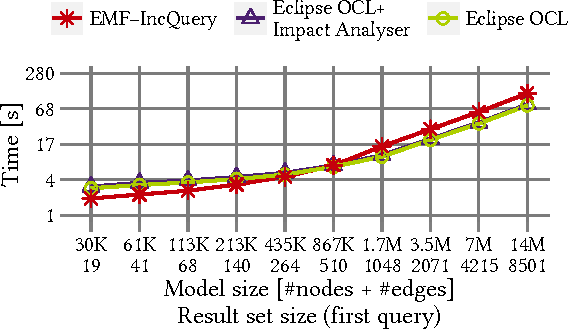
\includegraphics[width=0.9\textwidth]{figures/trainBenchmark_User_BatchValid_RouteSensor}
	    \caption{Batch Query Evaluation Time -- RouteSensor}
	    \label{fig:BatchValid_RouteSensor}
	\end{subfigure}
	\begin{subfigure}[t]{0.48\textwidth}\centering
	    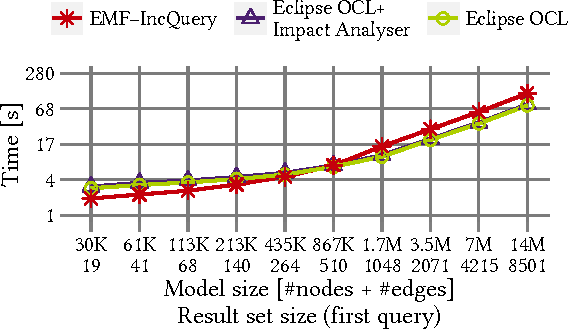
\includegraphics[width=0.9\textwidth]{figures/trainBenchmark_User_BatchValid_RouteSensor}
	    \caption{Batch Query Evaluation Time -- SignalNeighbor}
	    \label{fig:BatchValid_SignalNeighbor}
	\end{subfigure} \\

	\begin{subfigure}[t]{0.48\textwidth}\centering
	    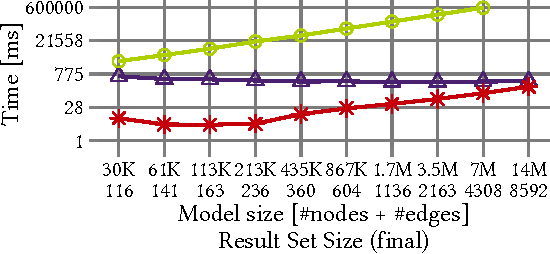
\includegraphics[width=0.9\textwidth]{figures/trainBenchmark_User_SumInc_RouteSensor}
	    \caption{Incremental Query Evaluation Time -- RouteSensor}
	    \label{fig:SumInc_RouteSensor}
	\end{subfigure}
	\begin{subfigure}[t]{0.48\textwidth}\centering
	    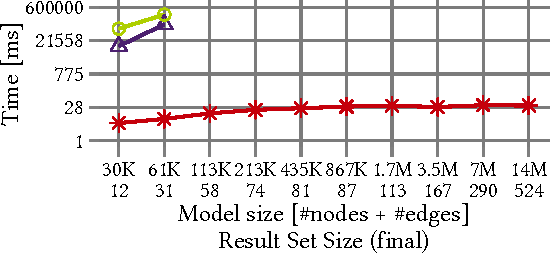
\includegraphics[width=0.9\textwidth]{figures/trainBenchmark_User_SumInc_SignalNeighbor}
	    \caption{Incremental Query Evaluation Time -- SignalNeighbor}
	    \label{fig:SumInc_SignalNeighbor}
	\end{subfigure} \\

	\begin{subfigure}[t]{0.48\textwidth}\centering
	    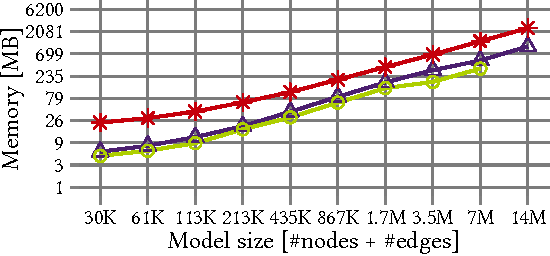
\includegraphics[width=0.9\textwidth]{figures/trainBenchmark_User_Memory_RouteSensor}
	    \caption{Memory Usage -- RouteSensor}
	    \label{fig:Memory_RouteSensor}
	\end{subfigure}
	\begin{subfigure}[t]{0.48\textwidth}\centering
	    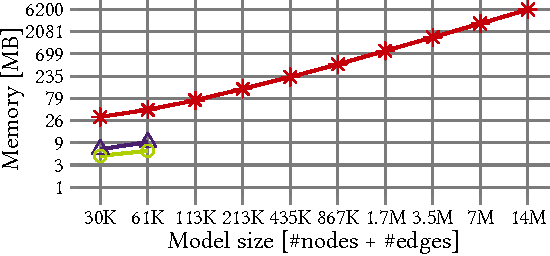
\includegraphics[width=0.9\textwidth]{figures/trainBenchmark_User_Memory_SignalNeighbor}
	    \caption{Memory Usage -- SignalNeighbor}
	    \label{fig:Memory_SignalNeighbor}
	\end{subfigure}
  \caption{Benchmark results.}
  \label{fig:trainbenchmark-diagrams}
\end{center}
\end{figure}

For the more complex \textsf{SignalNeighbor} query
\autoref{fig:BatchValid_SignalNeighbor} depicts that \incquery{} (somewhat
surprisingly) outperforms OCL solutions: it is noticeably faster for small
modells (2 s and 4 s), and over 435k model elements OCL did not finish with
the initial analysis in 12 minutes. This performance gain might be attributed to
the more efficient (cached) enumeration of instances, and the possibility of
backward navigation (with the help of auxiliary structures) on unidirectional
references used by this query.

\subsection{Incremental Query Evaluation}
In the \emph{incremental case}, Eclipse OCL evaluates the query on each run
(100 times) from scratch, its execution time increases linearly with
model size, resulting slow overall evaluation.

For the \textsf{RouteSensor} query (\autoref{fig:SumInc_RouteSensor}), the Impact
Analyzer performs the 100 modifications in 350 ms regardless of the model
size. On the same query, \incquery{} starts much faster, but its speed reduces
on the larger models (from 9 to 220 ms). On the other hand, the Impact
Analyzer is an order of magnitude slower on the \textsf{SignalNeighbor} query
(\autoref{fig:SumInc_SignalNeighbor}) query: it does not finish in 12 minutes
for models over 61k model elements, while \incquery{} handles every model
regardless of size under 40 ms.

The performance of the Impact Analyzer is most likely affected by the previously
mentioned unidirectional references. The slowdown of \incquery{} is probably
caused by the increased number of matches (from 116 to 8592), as query
results are always available in the output nodes of Rete networks, and only a
linear traversal of these stored matches is needed to return them.

\subsection{Threats to Validity}
We tried to mitigate \emph{internal validity} threats by reducing the number of
uncontrolled variables during measurements: a physical machine was used with all
unnecessary software components turned off and every execution was isolated into
a freshly initialized JVM.

The queries are semantically equivalent in the different query languages and the
result sets are the same for every model. Additionally, to ensure comparable
results the created high-quality query implementations were reviewed: the OCL
implementation by Ed Willink from the Eclipse OCL project, the usage of Impact
Analyzer by Axel Uhl from the Impact Analyzer developer team. The graph patterns
were written by the developers of \incquery{}.

Considering \emph{external validity}, the generalization of the results largely
depends on how representative the metamodels, the models and the queries are
compared to real use cases. In section \ref{specification-extended} metrics were
defined to describe complexity of models and queries, however comparing them to
real world ones remains a future work.

The metamodel and the query specifications were motivated by an industrial case
study, and the selected queries feature commonly used validation tasks such as
attribute and reference checks or cycle detection. We tried to ensure that the
instance models have a similar structure and distribution to other models by
parameterizing the generation process based on our experience with other
domains. To summarize, we believe that the train domain and the generated
instance models represent other domain-specific languages and available instance
models well.

Our current measurements only loaded and executed a single query in each run.
When loading multiple queries, query interference may change the results
greatly. A more detailed evaluation of this issue is planned for the future.

Considering resource-constrained environments, we believe that limiting
available memory will alter the results the most, as the memory management
overhead will reduce the performance of \incquery{}.

It is important to note that heap usage were measured after executing a garbage
collection, so these measurements do not contain memory usage of temporary
constructs. This means that maximum heap usage might have been larger. Furthermore,
limiting heap space by the maximum usage results in excessive garbage collection
and thus an increased runtime. However, in our experience setting the limit to
two times the measured values, such issues do not occur.

In case of the benchmark queries, we measured a $1.5$GB heap size in case of a
model with $3.5$M model elements that we believe is manageable in a developer
machine with $4$--$8$GB of RAM. On the other hand, when handling such large
models the existing user interface itself could become a bottleneck. Thus we
believe, our measurement results hold also in the integrated development
environments.
